\documentclass[journal]{IEEEtran} % use the `journal` option for ITherm conference style
\IEEEoverridecommandlockouts
% The preceding line is only needed to identify funding in the first footnote. If that is unneeded, please comment it out.
\usepackage{cite}
\usepackage{amsmath,amssymb,amsfonts}
\usepackage{algorithmic}
\usepackage{graphicx}
\usepackage{textcomp}
\usepackage{xcolor}
\usepackage{float} 
\usepackage{hyperref}

% Configuración de hyperref para enlaces en azul
\hypersetup{
    colorlinks=true,
    linkcolor=blue,
    urlcolor=blue,
    citecolor=blue
} 
\def\BibTeX{{\rm B\kern-.05em{\sc i\kern-.025em b}\kern-.08em
    T\kern-.1667em\lower.7ex\hbox{E}\kern-.125emX}}
\begin{document}

\title{Fundamentos de Señales Telefónicas y Codificación de Voz en Matlab \\
% delete or comment-out the following line before submission
%{\footnotesize \textsuperscript{*}Note: Sub-titles are not captured in Xplore and should not be used}
\thanks{Identify applicable funding agency here. If none, delete this.}
}

\author{%%%% author names
    \IEEEauthorblockN{Darwin Cristhian Turpo Quispe}% first author
    , \IEEEauthorblockN{Luque Llanqui Vladimir Williams}% second author
    , \IEEEauthorblockN{Maldonado Lima Roger Jhon}% third author
    % duplicate the line above as many times as needed to list all authors
    \\%%%% author affiliations
    \IEEEauthorblockA{\textit{Escuela Profesional de Ingeniería en Telecomunicaciones}}\\% first affiliation
    \IEEEauthorblockA{\textit{Universidad Nacional de San Agustín de Arequipa}}\\% second affiliation
    \IEEEauthorblockA{\textit{Repositorio: \href{https://github.com/DarwinTQ/lab_sistemas_telefonia/tree/main/lab01}{https://github.com/DarwinTQ/lab\_sistemas\_telefonia/tree/main/lab01}}}\\% repository
    % duplicate the line above as many times as needed to list all affiliations
    %%%% corresponding author contact details
    %\IEEEauthorblockA{email address or ORCID of corresponding author(s)}
}

\maketitle

% \begin{abstract}
%     This document is a model and instructions for \LaTeX.
%     This and the IEEEtran.cls file define the components of your paper [title, text, heads, etc.]. *CRITICAL: Do Not Use Symbols, Special Characters, Footnotes,
%     or Math in Paper Title or Abstract.
% \end{abstract}

% \begin{IEEEkeywords}
%     component, formatting, style, styling, insert
% \end{IEEEkeywords}

\section{Introducción}
La transición de la telefonía analógica a la digital se basa en principios de procesamiento de señales que garantizan la eficiencia y calidad de la comunicación. Dos de los pilares de esta tecnología son la señalización DTMF para la marcación y la modulación PCM para la digitalización de la voz.

El objetivo de este laboratorio es comprender y simular estos fundamentos. Primero, se aborda la generación de tonos DTMF, visualizando su composición como la suma de dos sinusoides y verificando sus componentes espectrales. Segundo, se explora el proceso de digitalización de una señal de voz mediante PCM, analizando los efectos del error de cuantización. Finalmente, se compara la cuantización uniforme con la no uniforme, implementada a través de la técnica de companding Ley-A, para evaluar su impacto en la calidad de la señal de voz mediante métricas objetivas (SNQ) y subjetivas (MOS).

\section{Marco Teórico}

\subsection{Tonos DTMF (Dual-Tone Multi-Frequency)}
Sistema de señalización por tonos utilizado en telefonía donde cada dígito está representado por dos tonos sinusoidales simultáneos:
\begin{itemize}
    \item Frecuencias bajas: 697, 770, 852, 941 Hz
    \item Frecuencias altas: 1209, 1336, 1477, 1633 Hz
\end{itemize}

\subsection{Modulación PCM (Pulse Code Modulation)}
Proceso de digitalización de señales analógicas:
\begin{itemize}
    \item Muestreo: $f_s \geq 2f_{max}$ (Teorema de Nyquist)
    \item Cuantización: $Q = \frac{2^N - 1}{A}$
    \item Codificación: Representación binaria
\end{itemize}

\subsection{Companding}
Técnica de compresión-expansión:
\begin{itemize}
    \item Ley A: $y = \frac{1 + \ln(A)}{A}|x|$ para $|x| < \frac{1}{A}$
    \item Ley $\mu$: $y = \frac{\ln(1 + \mu)}{\ln(1 + \mu|x|)}$
\end{itemize}

\subsection{Métricas de Calidad}
\begin{itemize}
    \item SNQ: $SNQ = 10\log_{10}\left(\frac{P_{\text{señal}}}{P_{\text{error}}}\right)$
    \item MOS: Escala subjetiva 1-5
\end{itemize}

\section{Desarrollo}
% Before you begin to format your paper, first write and save the content as a
% separate text file. Complete all content and organizational editing before
% formatting. Please note sections \ref{AA}--\ref{SCM} below for more information on
% proofreading, spelling and grammar.

% Keep your text and graphic files separate until after the text has been
% formatted and styled. Do not number text heads---{\LaTeX} will do that
% for you.

\subsection{Generación y Análisis de Tonos DTMF}\label{AA}
Los parámetros iniciales, como una frecuencia de muestreo $f_s=8000$ Hz y una duración de 0.5 segundos por tono.

\begin{table}[htbp]
    \caption{Matriz de Frecuencias DTMF}
    \begin{center}
        \begin{tabular}{|c|c|c|c|c|}
            \hline
            \textbf{} & \textbf{1209 Hz} & \textbf{1336 Hz} & \textbf{1477 Hz} & \textbf{1633 Hz} \\
            \hline
            \textbf{697 Hz} & 1 & 2 & 3 & A \\
            \hline
            \textbf{770 Hz} & 4 & 5 & 6 & B \\
            \hline
            \textbf{852 Hz} & 7 & 8 & 9 & C \\
            \hline
            \textbf{941 Hz} & * & 0 & \# & D \\
            \hline
        \end{tabular}
        \label{tab:dtmf}
    \end{center}
\end{table}


\subsection{Modulación PCM y Codificación de Voz}

\textbf{Carga de Señal:} Se cargó un archivo de audio `voz\_prueba.wav` o, en su defecto, se generó una señal sintética. La señal fue normalizada.

\textbf{PCM Uniforme:} Se aplicó cuantización uniforme a la señal de voz utilizando diferentes resoluciones: 4, 8 y 12 bits. Se comparó gráficamente la señal original con la señal cuantizada.

\textbf{PCM con Companding Ley-A:} La señal de voz original fue primero comprimida usando la Ley-A con un valor estándar de $A=87.6$. Posteriormente, se aplicó una cuantización uniforme de 8 bits a la señal comprimida.

\textbf{Evaluación de Calidad:} Se calculó y comparó la SNQ para la PCM uniforme de 8 bits y para la PCM de 8 bits con companding Ley-A. Con base en los valores de SNQ, se estimó una puntuación MOS para cada caso.

\textbf{Análisis Espectral y Auditivo:} Finalmente, se reprodujeron las señales de audio (original, PCM uniforme y PCM con companding) para una comparación auditiva y se graficaron sus respectivos espectros de frecuencia.

% \subsection{Equations}
% Number equations consecutively. To make your
% equations more compact, you may use the solidus (~/~), the exp function, or
% appropriate exponents. Italicize Roman symbols for quantities and variables,
% but not Greek symbols. Use a long dash rather than a hyphen for a minus
% sign. Punctuate equations with commas or periods when they are part of a
% sentence, as in:
% \begin{equation}
%     a+b=\gamma\label{eq}
% \end{equation}

% Be sure that the
% symbols in your equation have been defined before or immediately following
% the equation. Use ``\eqref{eq}'', not ``Eq.~\eqref{eq}'' or ``equation \eqref{eq}'', except at
% the beginning of a sentence: ``Equation \eqref{eq} is . . .''

% \subsection{\LaTeX-Specific Advice}

% Please use ``soft'' (e.g., \verb|\eqref{Eq}|) cross references instead
% of ``hard'' references (e.g., \verb|(1)|). That will make it possible
% to combine sections, add equations, or change the order of figures or
% citations without having to go through the file line by line.

% Please don't use the \verb|{eqnarray}| equation environment. Use
% \verb|{align}| or \verb|{IEEEeqnarray}| instead. The \verb|{eqnarray}|
% environment leaves unsightly spaces around relation symbols.

% Please note that the \verb|{subequations}| environment in {\LaTeX}
% will increment the main equation counter even when there are no
% equation numbers displayed. If you forget that, you might write an
% article in which the equation numbers skip from (17) to (20), causing
% the copy editors to wonder if you've discovered a new method of
% counting.

%     {\BibTeX} does not work by magic. It doesn't get the bibliographic
% data from thin air but from .bib files. If you use {\BibTeX} to produce a
% bibliography you must send the .bib files.

%     {\LaTeX} can't read your mind. If you assign the same label to a
% subsubsection and a table, you might find that Table I has been cross
% referenced as Table IV-B3.

% {\LaTeX} does not have precognitive abilities. If you put a
% \verb|\label| command before the command that updates the counter it's
% supposed to be using, the label will pick up the last counter to be
% cross referenced instead. In particular, a \verb|\label| command
% should not go before the caption of a figure or a table.

% Do not use \verb|\nonumber| inside the \verb|{array}| environment. It
% will not stop equation numbers inside \verb|{array}| (there won't be
% any anyway) and it might stop a wanted equation number in the
% surrounding equation.

% \subsection{Some Common Mistakes}\label{SCM}
% \begin{itemize}
%     \item The word ``data'' is plural, not singular.
%     \item The subscript for the permeability of vacuum $\mu_{0}$, and other common scientific constants, is zero with subscript formatting, not a lowercase letter ``o''.
%     \item In American English, commas, semicolons, periods, question and exclamation marks are located within quotation marks only when a complete thought or name is cited, such as a title or full quotation. When quotation marks are used, instead of a bold or italic typeface, to highlight a word or phrase, punctuation should appear outside of the quotation marks. A parenthetical phrase or statement at the end of a sentence is punctuated outside of the closing parenthesis (like this). (A parenthetical sentence is punctuated within the parentheses.)
%     \item A graph within a graph is an ``inset'', not an ``insert''. The word alternatively is preferred to the word ``alternately'' (unless you really mean something that alternates).
%     \item Do not use the word ``essentially'' to mean ``approximately'' or ``effectively''.
%     \item In your paper title, if the words ``that uses'' can accurately replace the word ``using'', capitalize the ``u''; if not, keep using lower-cased.
%     \item Be aware of the different meanings of the homophones ``affect'' and ``effect'', ``complement'' and ``compliment'', ``discreet'' and ``discrete'', ``principal'' and ``principle''.
%     \item Do not confuse ``imply'' and ``infer''.
%     \item The prefix ``non'' is not a word; it should be joined to the word it modifies, usually without a hyphen.
%     \item There is no period after the ``et'' in the Latin abbreviation ``et al.''.
%     \item The abbreviation ``i.e.'' means ``that is'', and the abbreviation ``e.g.'' means ``for example''.
% \end{itemize}
% An excellent style manual for science writers is \cite{b7}.

% \subsection{Authors and Affiliations}
% \textbf{The class file is designed for, but not limited to, six authors.} A
% minimum of one author is required for all conference articles. Author names
% should be listed starting from left to right and then moving down to the
% next line. This is the author sequence that will be used in future citations
% and by indexing services. Names should not be listed in columns nor group by
% affiliation. Please keep your affiliations as succinct as possible (for
% example, do not differentiate among departments of the same organization).

% \subsection{Identify the Headings}
% Headings, or heads, are organizational devices that guide the reader through
% your paper. There are two types: component heads and text heads.

% Component heads identify the different components of your paper and are not
% topically subordinate to each other. Examples include Acknowledgments and
% References and, for these, the correct style to use is ``Heading 5''. Use
% ``figure caption'' for your Figure captions, and ``table head'' for your
% table title. Run-in heads, such as ``Abstract'', will require you to apply a
% style (in this case, italic) in addition to the style provided by the drop
% down menu to differentiate the head from the text.

% Text heads organize the topics on a relational, hierarchical basis. For
% example, the paper title is the primary text head because all subsequent
% material relates and elaborates on this one topic. If there are two or more
% sub-topics, the next level head (uppercase Roman numerals) should be used
% and, conversely, if there are not at least two sub-topics, then no subheads
% should be introduced.

% \subsection{Figures and Tables}
% \paragraph{Positioning Figures and Tables} Place figures and tables at the top and
% bottom of columns. Avoid placing them in the middle of columns. Large
% figures and tables may span across both columns. Figure captions should be
% below the figures; table heads should appear above the tables. Insert
% figures and tables after they are cited in the text. Use the abbreviation
% ``Fig.~\ref{fig}'', even at the beginning of a sentence.

% \begin{table}[htbp]
%     \caption{Table Type Styles}
%     \begin{center}
%         \begin{tabular}{|c|c|c|c|}
%             \hline
%             \textbf{Table} & \multicolumn{3}{|c|}{\textbf{Table Column Head}}                                                         \\
%             \cline{2-4}
%             \textbf{Head}  & \textbf{\textit{Table column subhead}}           & \textbf{\textit{Subhead}} & \textbf{\textit{Subhead}} \\
%             \hline
%             copy           & More table copy$^{\mathrm{a}}$                   &                           &                           \\
%             \hline
%             \multicolumn{4}{l}{$^{\mathrm{a}}$Sample of a Table footnote.}
%         \end{tabular}
%         \label{tab1}
%     \end{center}
% \end{table}

% \begin{figure}[htbp]
%     \centerline{
\includegraphics{fig1.png}}
%     \caption{Example of a figure caption.}
%     \label{fig}
% \end{figure}

% Figure Labels: Use 8 point Times New Roman for Figure labels. Use words
% rather than symbols or abbreviations when writing Figure axis labels to
% avoid confusing the reader. As an example, write the quantity
% ``Magnetization'', or ``Magnetization, M'', not just ``M''. If including
% units in the label, present them within parentheses. Do not label axes only
% with units. In the example, write ``Magnetization (A/m)'' or ``Magnetization
% \{A[m(1)]\}'', not just ``A/m''. Do not label axes with a ratio of
% quantities and units. For example, write ``Temperature (K)'', not
% ``Temperature/K''.

\section{Resultados}

\subsection{Análisis de Tonos DTMF}\label{AA}
% insertar un parrafo
La figura 1 muestra la forma de onda de la señal DTMF para el dígito '5' en el dominio del tiempo. Se observa una señal periódica compleja, resultado de la suma de dos sinusoides.
\begin{figure}[H]
    \centerline{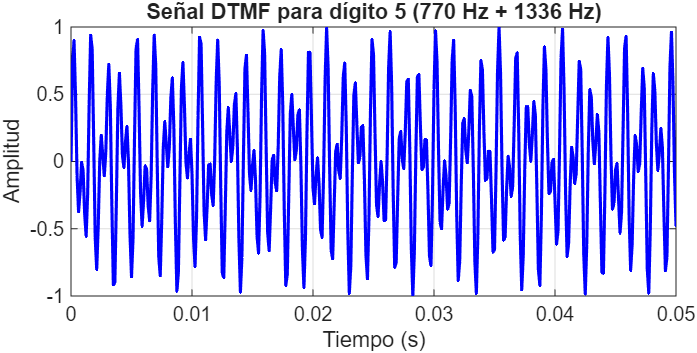
\includegraphics[width=0.8\columnwidth]{Figure_1.png}}
    \caption{Forma de onda DTMF para el dígito '5'.}
    \label{fig}
\end{figure}

%este texto tiene que estar despues de la fig 1 y antes de la fig 2

La figura 2 muestra el espectro de frecuencias de la señal DTMF para el dígito '5'. Se identifican claramente los picos en las frecuencias correspondientes a 770 Hz y 1336 Hz, confirmando la composición dual-tone de la señal.

\begin{figure}[H]
    \centerline{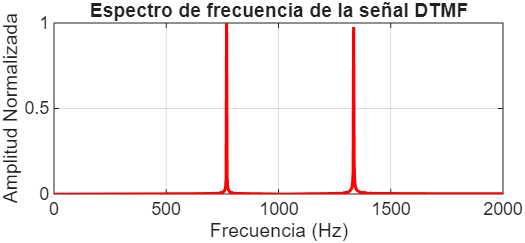
\includegraphics[width=0.8\columnwidth]{Figure_2.png}}
    \caption{Espectro de frecuencias DTMF para el dígito '5'.}
    \label{fig}
\end{figure}

La figura 3 muestra la forma de onda de la señal DTMF para el dígito '1' en el dominio del tiempo. Se observa una señal periódica compleja, resultado de la suma de dos sinusoides.

\begin{figure}[H]
    \centerline{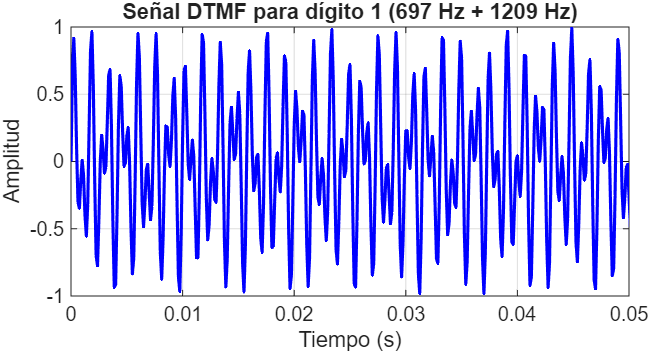
\includegraphics[width=0.8\columnwidth]{Figure_3.png}}
    \caption{Forma de onda DTMF para el dígito '1'.}
    \label{fig}
\end{figure}


La figura 4 muestra el espectro de frecuencias de la señal DTMF para el dígito '1'. Se identifican claramente los picos en las frecuencias correspondientes a 697 Hz y 1209 Hz, confirmando la composición dual-tone de la señal.
\begin{figure}[H]
    \centerline{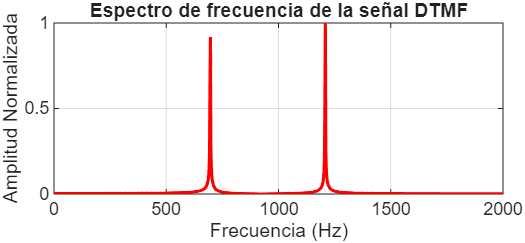
\includegraphics[width=0.8\columnwidth]{Figure_4.png}}
    \caption{Espectro de frecuencias DTMF para el dígito '1'.}
    \label{fig}
\end{figure}


La figura 5 muestra la forma de onda de la señal DTMF para el dígito 'C' en el dominio del tiempo. Se observa una señal periódica compleja, resultado de la suma de dos sinusoides.
\begin{figure}[H]
    \centerline{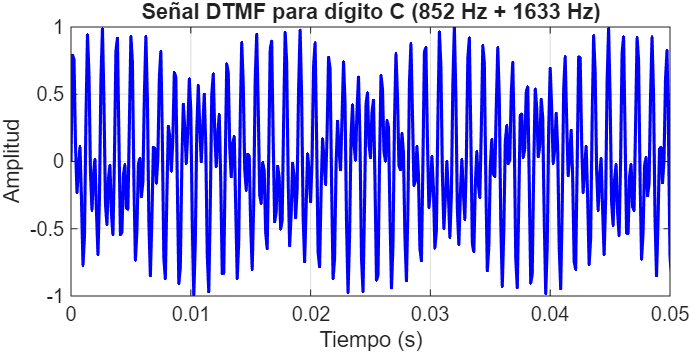
\includegraphics[width=0.8\columnwidth]{Figure_5.png}}
    \caption{Forma de onda DTMF para el dígito 'C'.}
    \label{fig}
\end{figure}


La figura 6 muestra el espectro de frecuencias de la señal DTMF para el dígito 'C'. Se identifican claramente los picos en las frecuencias correspondientes a 852 Hz y 1477 Hz, confirmando la composición dual-tone de la señal.
\begin{figure}[H]
    \centerline{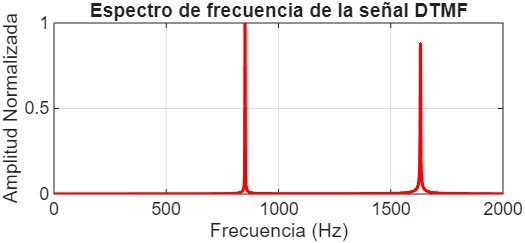
\includegraphics[width=0.8\columnwidth]{Figure_6.png}}
    \caption{Espectro de frecuencias DTMF para el dígito 'C'.}
    \label{fig} 
\end{figure}


\subsection{Modulación PCM y Codificación de Voz}
Creacion del archivo de audio voz\_prueba.wav con una señal de voz sintetica.
\begin{verbatim}
    === GRABADORA DE VOZ ===
Frecuencia: 8000 Hz
Duración: 5 segundos
Archivo: voz_prueba.wav

Preparando grabación...
Grabando durante 5 segundos...
HABLE AHORA...
Grabación completada.
Archivo guardado: voz_prueba.wav
Duración: 5.00 segundos
Muestras: 40000
Error al guardar el archivo: Unrecognized field name "FileSize".

¿Reproducir grabación? (s/n): s
Reproduciendo...

=== PROCESO COMPLETADO ===
El archivo voz_prueba.wav está listo para usar.

\end{verbatim}

MODULACIÓN PCM Y CODIFICACIÓN DE VOZ
\begin{verbatim}
    El archivo voz_prueba.wav está listo para usar.
SNQ PCM Uniforme 8-bit: 39.88 dB
SNQ PCM + Companding A-law 8-bit: -3.09 dB
Reproduciendo voz original...
Reproduciendo voz con PCM uniforme 8-bit...
Reproduciendo voz con companding A-law...

--- CALIDAD DE VOZ ESTIMADA ---
PCM Uniforme 8-bit: MOS = 4.5
PCM + Companding: MOS = 2.5
>> parte2
SNQ PCM Uniforme 8-bit: 39.88 dB
SNQ PCM + Companding A-law 8-bit: -3.09 dB
Reproduciendo voz original...
Reproduciendo voz con PCM uniforme 8-bit...
Reproduciendo voz con companding A-law...

--- CALIDAD DE VOZ ESTIMADA ---
PCM Uniforme 8-bit: MOS = 4.5
PCM + Companding: MOS = 2.5
>> 

\end{verbatim}

La figura 7 muestra PCM uniforme con 4, 8 y 12 bits respectivamente. Se observa que a medida que aumenta la cantidad de bits, la señal cuantizada se aproxima más a la señal original, reduciendo el error de cuantización.
\begin{figure}[H]
    \centerline{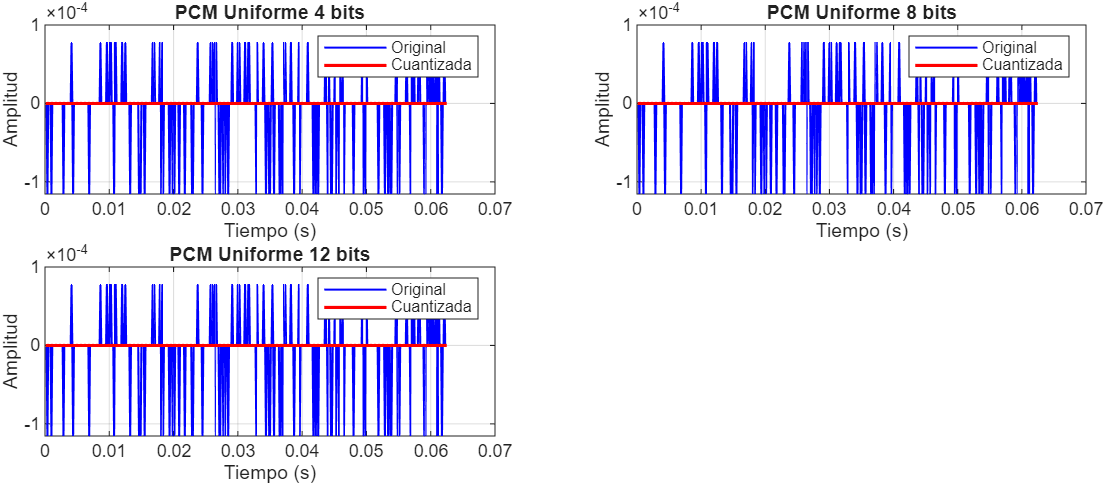
\includegraphics[width=0.8\columnwidth]{Figure_7.png}}
    \caption{PCM uniforme con 4, 8 y 12 bits.}
    \label{fig} 
\end{figure}

La figura 8 muestra Especro voz original, espectro PCM uniforme 8 bits, espectro error de cuantización y espectro PCM + companding A -law. Se observa que la PCM con companding A-law presenta un espectro más cercano al de la señal original, indicando una mejor preservación de las características de la voz.
\begin{figure}[H]
    \centerline{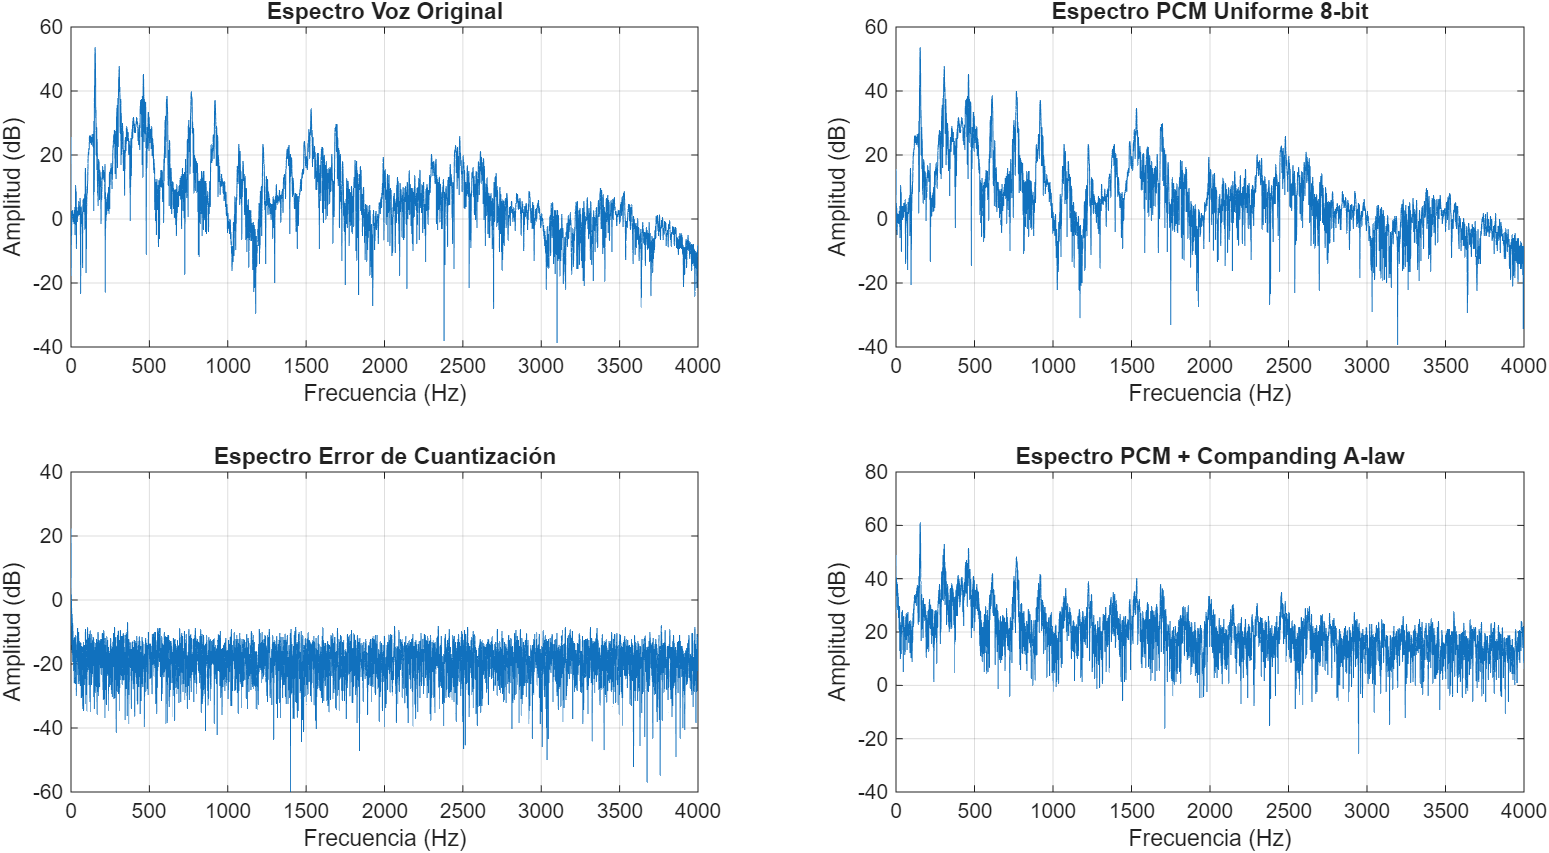
\includegraphics[width=0.8\columnwidth]{Figure_8.png}}
    \caption{Espectros de voz original, PCM uniforme 8 bits, error de cuantización y PCM + companding A-law.}
    \label{fig} 
\end{figure}








\section{Conclusiones}

\begin{itemize}
    \item Se comprobó que la señalización DTMF funciona mediante la combinación de dos frecuencias específicas, lo que permite identificar de manera única cada dígito telefónico.
    
    \item En la modulación PCM, se verificó que el número de bits de cuantización influye directamente en la calidad de la señal digitalizada: a mayor número de bits, menor error y mejor calidad de voz.
    
    \item El uso de técnicas de companding (Ley A o Ley $\mu$) mejora la relación señal/ruido de cuantización y permite obtener una mejor calidad percibida sin necesidad de incrementar el número de bits.
    
    \item Se comprobó que la elección de la frecuencia de muestreo ($f_s$) es crítica para evitar aliasing. Esto confirma lo establecido por el teorema de Nyquist-Shannon, que asegura una reconstrucción fiel de la señal cuando $f_s \geq 2f_{max}$.
    
    \item El laboratorio permitió comprender de manera práctica cómo los procesos de muestreo y cuantización influyen directamente en la calidad del audio digital. Se comprobó que una reducción en el número de bits de cuantización genera un incremento en el error y en la distorsión de la señal, afectando la fidelidad de la voz y su inteligibilidad.
\end{itemize}



% \section*{Acknowledgment}

% The preferred spelling of the word ``acknowledgment'' in America is without
% an ``e'' after the ``g''. Avoid the stilted expression ``one of us (R. B.
% G.) thanks $\ldots$''. Instead, try ``R. B. G. thanks$\ldots$''. Put sponsor
% acknowledgments in the unnumbered footnote on the first page.

% \section*{References}

% Please number citations consecutively within brackets \cite{b1}. The
% sentence punctuation follows the bracket \cite{b2}. Refer simply to the reference
% number, as in \cite{b3}---do not use ``Ref. \cite{b3}'' or ``reference \cite{b3}'' except at
% the beginning of a sentence: ``Reference \cite{b3} was the first $\ldots$''

% Number footnotes separately in superscripts. Place the actual footnote at
% the bottom of the column in which it was cited. Do not put footnotes in the
% abstract or reference list. Use letters for table footnotes.

% Unless there are six authors or more give all authors' names; do not use
% ``et al.''. Papers that have not been published, even if they have been
% submitted for publication, should be cited as ``unpublished'' \cite{b4}. Papers
% that have been accepted for publication should be cited as ``in press'' \cite{b5}.
% Capitalize only the first word in a paper title, except for proper nouns and
% element symbols.

% For papers published in translation journals, please give the English
% citation first, followed by the original foreign-language citation \cite{b6}.

\begin{thebibliography}{00}
    \bibitem{b1} IEEE, ``IEEE Conference Templates,'' [En línea]. Disponible en: https://www.ieee.org/conferences/publishing/templates. [Accedido: 16 sep. 2025].
    \bibitem{b2} MathWorks, ``MATLAB Graphics Documentation,'' [En línea]. Disponible en: https://la.mathworks.com/help/matlab/graphics.html. [Accedido: 16 sep. 2025].
    \bibitem{b3} Anthropic, ``Claude AI Assistant,'' [En línea]. Disponible en: https://claude.ai. [Accedido: 16 sep. 2025].
\end{thebibliography}
\vspace{12pt}
% \color{red}
% IEEE conference templates contain guidance text for composing and formatting conference papers. Please ensure that all template text is removed from your conference paper prior to submission to the conference. Failure to remove the template text from your paper may result in your paper not being published.

\end{document}
